\documentclass[a4paper,12pt]{article}

\usepackage{graphicx}          % permite incluir eps no documento
%\usepackage[latin1]{inputenc}  % permite escrever com acentos
\usepackage{latexsym}
\usepackage{amssymb}           % carrega letras matem�ticas
\usepackage{mathrsfs}          % carrega letras matem�ticas
%\usepackage[english,american,portuges]{babel} % estrutura em portugues
\usepackage{hyperref}

\newcommand{\lead}{\textsc{\footnotesize LEAD}}

\newcommand{\win}{\textsc{\footnotesize WIN}}

\newcommand{\anp}{\textsc{\footnotesize ANP}}

\begin{document}

\section{Drama in Race Games}


Drama is a subjective measure concerning the quality of a board game. Mark Thompson [ref] in his seminal article defined \textit{drama} in the following way:

\begin{quote}
\begin{footnotesize} [...] it should be possible for a player to recover from a weaker position and still win the game. Victory should not be achievable in a single successful blow; the suspense should continue through an extended campaign. Otherwise an early disadvantage makes the remainder of the game uninteresting: the doomed player rightly guesses that the puzzle he is trying to solve has no solution and that thinking about it is futile. A game's drama might be measured roughly by matching a strong player against a weak player, and having them switch sides after the strong player achieves an advantage. In a dramatic game the strong player will still have a chance of winning.
\end{footnotesize}
\end{quote}

Thompson's text focused mainly on perfect-information games. However, we consider that the concept is also relevant in games were the random factor replaces the player's skill. Flipping a coin seems fundamentally less dramatic than playing the Game of Goose. So, it might make sense to define some criteria of drama, and apply it at race games, in order to measure and compare them. 

The strong random element in race games, instead of being an extra difficulty for analysis, provides an opportunity to measure drama using probabilistic tools. Instead of focusing in criteria that would provide a concrete number summarizing some pattern from the game rule structure, we will focus on concepts like averages and standard deviations that will naturally arise from playing many matches. This allows us to replace mathematical analysis with computational simulations.

Taking this into account, the authors reached the following statistical criteria for drama:

\begin{itemize}
	\setlength{\itemsep}{-2pt}
  	\setlength{\topsep}{-2pt}
	\item How balanced are the player's winning percentages? Given $n$ players, let's define \win~has the standard deviation of the estimated winning percentages of the first, second, third, ..., players. If they are all equal, then \win~will be zero. If there is high fluctuations in these estimates (e.g., the first player has a great advantage by starting first), then \win~will increase. A more balanced game allows for more dramatic matches, since the element of surprise of who will win increases with it.
	\item The amount of turns the winner had the lead just before winning, let's denote it \lead. If \lead~is, on average, very high, it means that the last turns on a race game lack novelty and tension. The leader just keeps leading until the game is over. On the other hand, if \lead~is low, last turn surprises will be common, and playing drama will occur often.
	\item The average number of players, \anp, that take the lead during a match at the end of an entire turn (i.e., after all players' moves). This measure makes more sense for game with a reasonable number of players (say, at least five players). Naturally, a low \anp~means very few players were on the lead, which is bad for dramatic matches. But also, a very high \anp~might also not be good. If, on average, almost all players take the lead, that means the game is not very decisive, and there is little tension in the initial stages, since players now that, on average, all will be ahead sometime. This would also imply very long matches (as always, on average). It seems appropriate that, for $n$ players, \anp~should be a middle value between $1$ and $n$.
\end{itemize}

\section{The Goose Experience}

\subsection{The experimental setup}

Herein we consider race games of the Game of Goose family. These games all share the following features:

\begin{itemize}
	\setlength{\itemsep}{-2pt}
  	\setlength{\topsep}{-2pt}
	\item Each player has one token that moves accordingly to the throw of two dice
	\item Each space in the board can only be occupied by a single token
	\item If a token lands on a previously occupied space, the two tokens switch their initial positions
	\item A token can only end the game if, in the last turn, the dice sum is the exact number needed to reach the final space
\end{itemize}

The games tested were the Game of Goose, the Game of the Universe and the Game of Navy. We will denote these three games as \textit{historical variants}. We also included an \textit{abstract variant}, that uses a board of 63 spaces like in the game of Goose and Navy, without any special rules (no traps, no jump spaces, etc.). This abstract variant is useful as a kind of control group to check the impact of the special rulings that characterizes every historical variant.

A program was implemented, written in the statistical R language, to automatically play these Goose-like games\footnote{The source code can be accessed at https://github.com/jpneto}. 

We performed multiple trials for each game. A \textit{trial} consists of 40000 matches played by the computer. We performed 12~trials for each one of the historical variants, and 6~trials for the abstract variant for a given number of players. For each variant, we played matches from three players up to eight players. The number of total matches played was over 10~million. This large amount was intended to decrease the probability of finding spurious patterns due to random noise effects.

For each trial a number of statistics were gathered for posterior analysis in order to estimate values for \lead, \win, \anp~drama criteria. The next sub-sections summarize these results.

\subsection{\win~criteria}

The \win~criteria deals with how balanced the variants are concerning winner percentages for each player. The plot at figure~\ref{fig:win_values} shows the results obtained by the match simulations performed by our software.

\begin{figure}[h!]
    % more info at https://www.sharelatex.com/learn/Inserting_Images
	\centering
	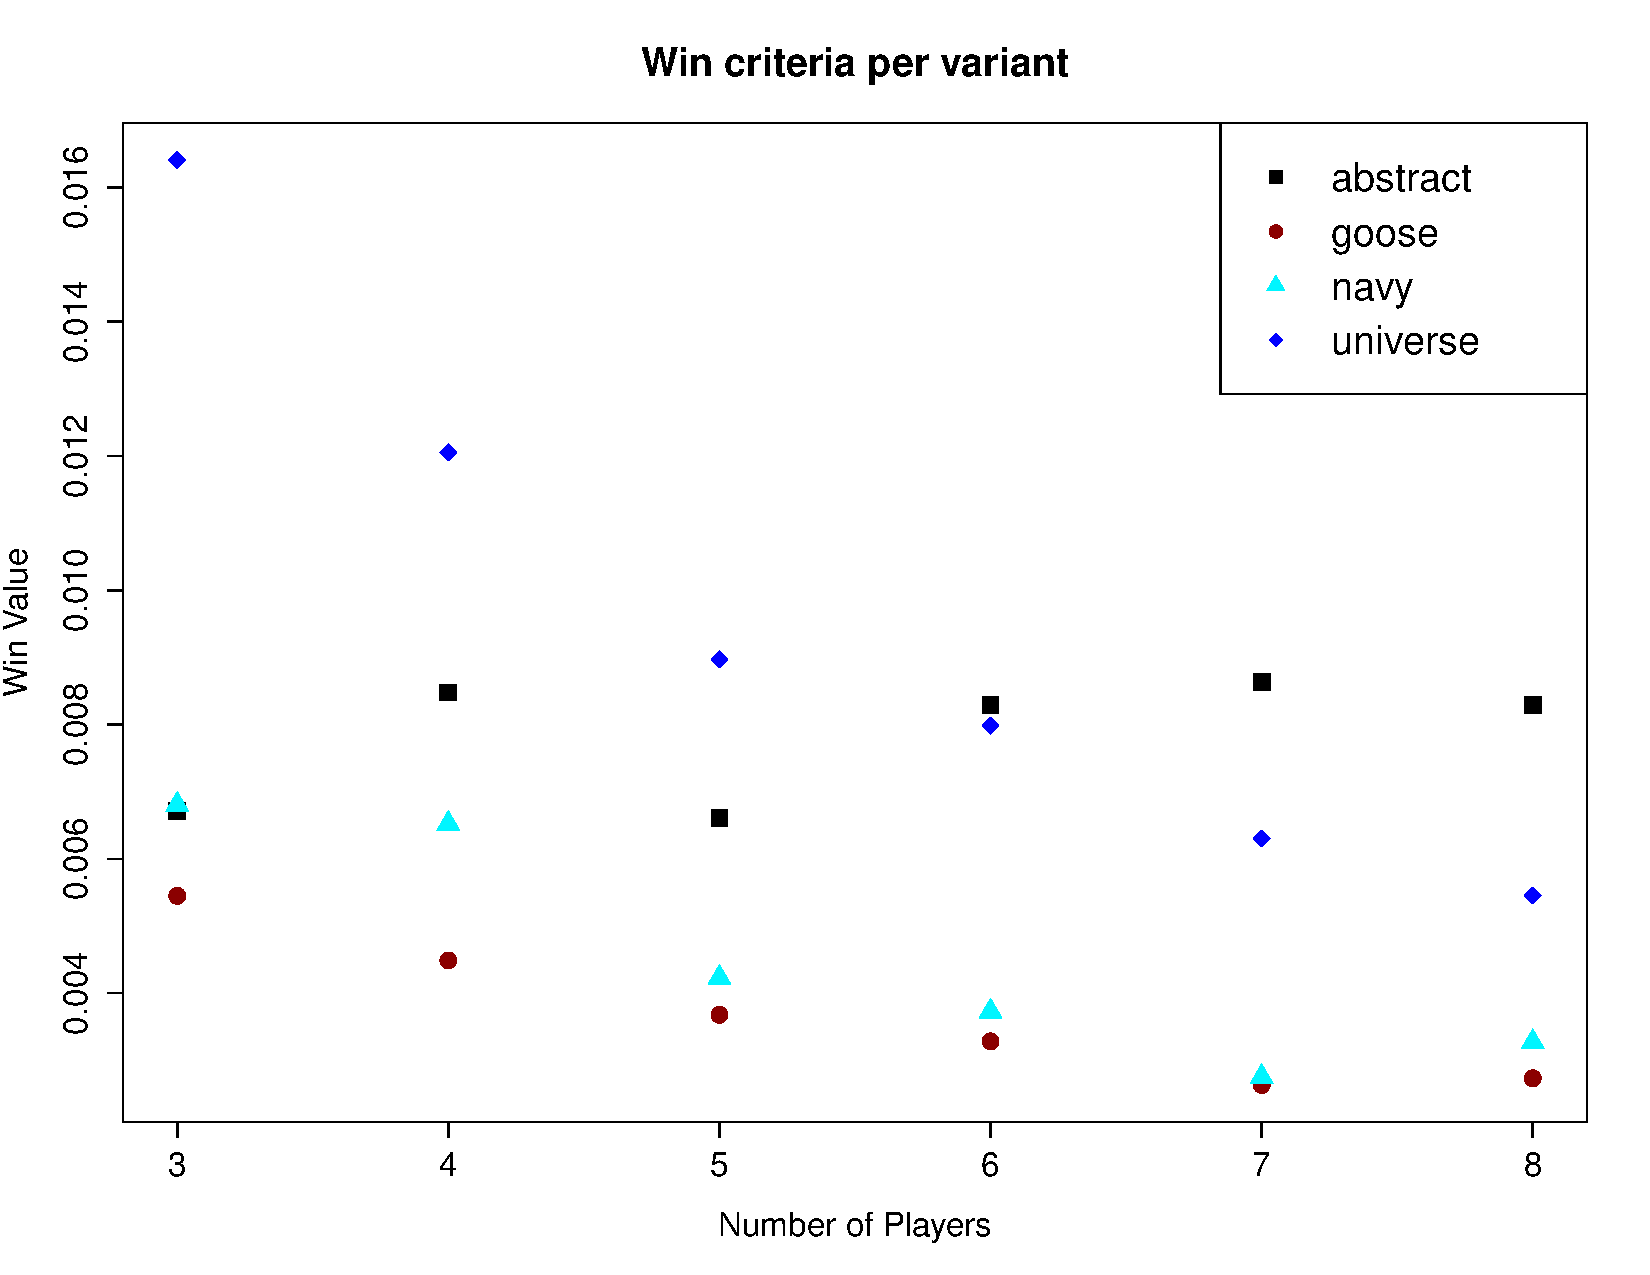
\includegraphics[scale=0.45]{imgs/win_plot.pdf}
	\caption{\small This plot shows the values of \win~for each variant -- each identified by a specific color and point shape -- and for each number of players. The \win~values are the standard deviation of the mean winner percentages of the respective game trials.}
    \label{fig:win_values}
\end{figure}

All historical games show a decrease in variation as the number of players increase. This means higher levels of drama with more players according to \win~criteria. The same effect does not happen in the abstract version. This indicates that the special rules typical of the historical variants do play a relevant role in adding drama to the overall gaming experience.

The game of Goose achieves the best \win~values for every number of players. The game of Navy achieves similar results. The other two games produce a larger variation. Notice however the small \win~values, almost all between $0.004$ and $0.009$. There are only two outliers for the Game of Universe with three and four players. These are values quite close to zero. To provide some context, a game with four players where the first two players had chances of victory of $26\%$ and the third and fourth players had $24\%$, the \win~value would be $0.012$.

There appears to be a curious inflexion point at seven players. Adding an eighth player seems to increase the variation if only slightly for the game of Goose and Navy. This might be a consequence of the board size. Both games have $63$~spaces and possibly the game becomes too crowded. That inflection does not happen for the game of Universe, which has larger board of 70 spaces. We speculate that its inflection point -- if indeed, this inflection is not just a product of statistical noise -- will occur by adding a ninth of tenth player.

Higher \win~values means that some players are winning more than others. Figure~\ref{fig:win_percents} shows which players are getting more wins:

\begin{figure}[h!]
	\centering
	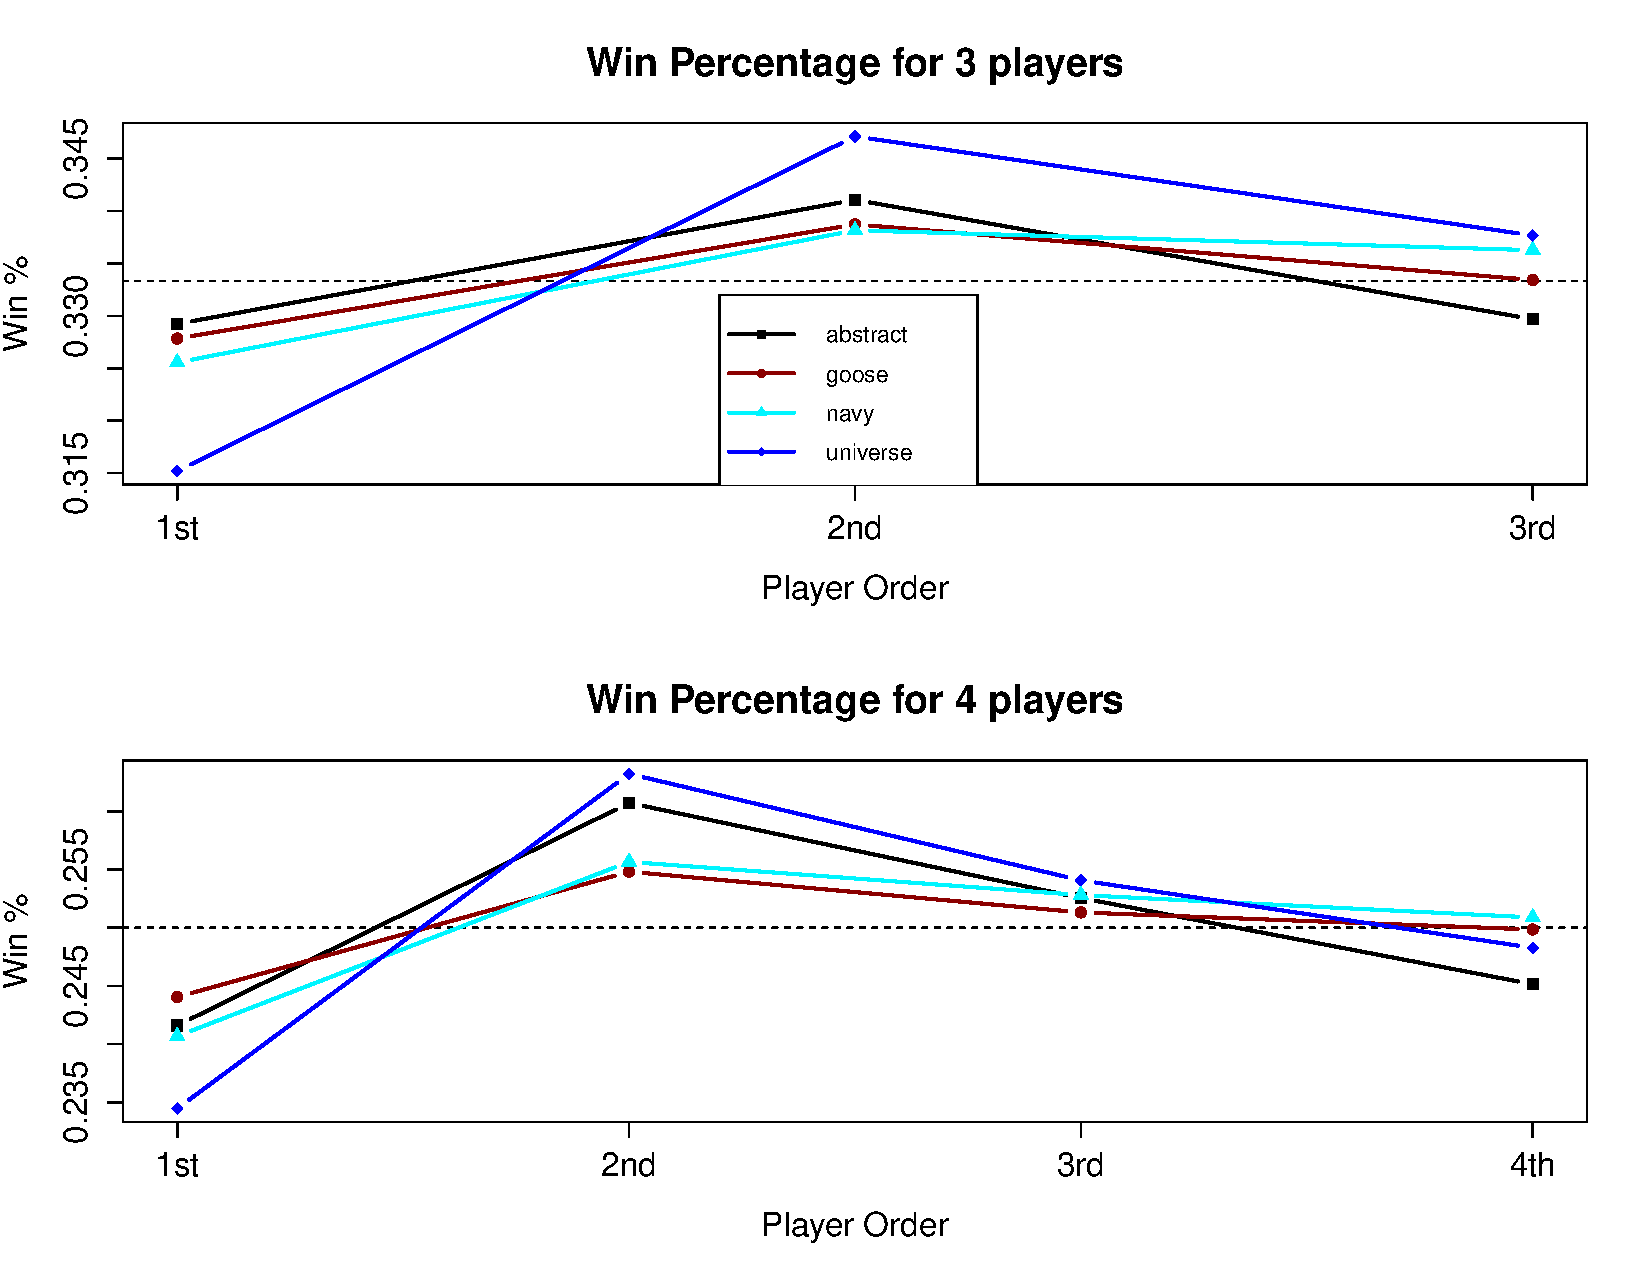
\includegraphics[scale=0.45]{imgs/win_3_4.pdf}
\end{figure}

\begin{figure}[h!]
	\centering
	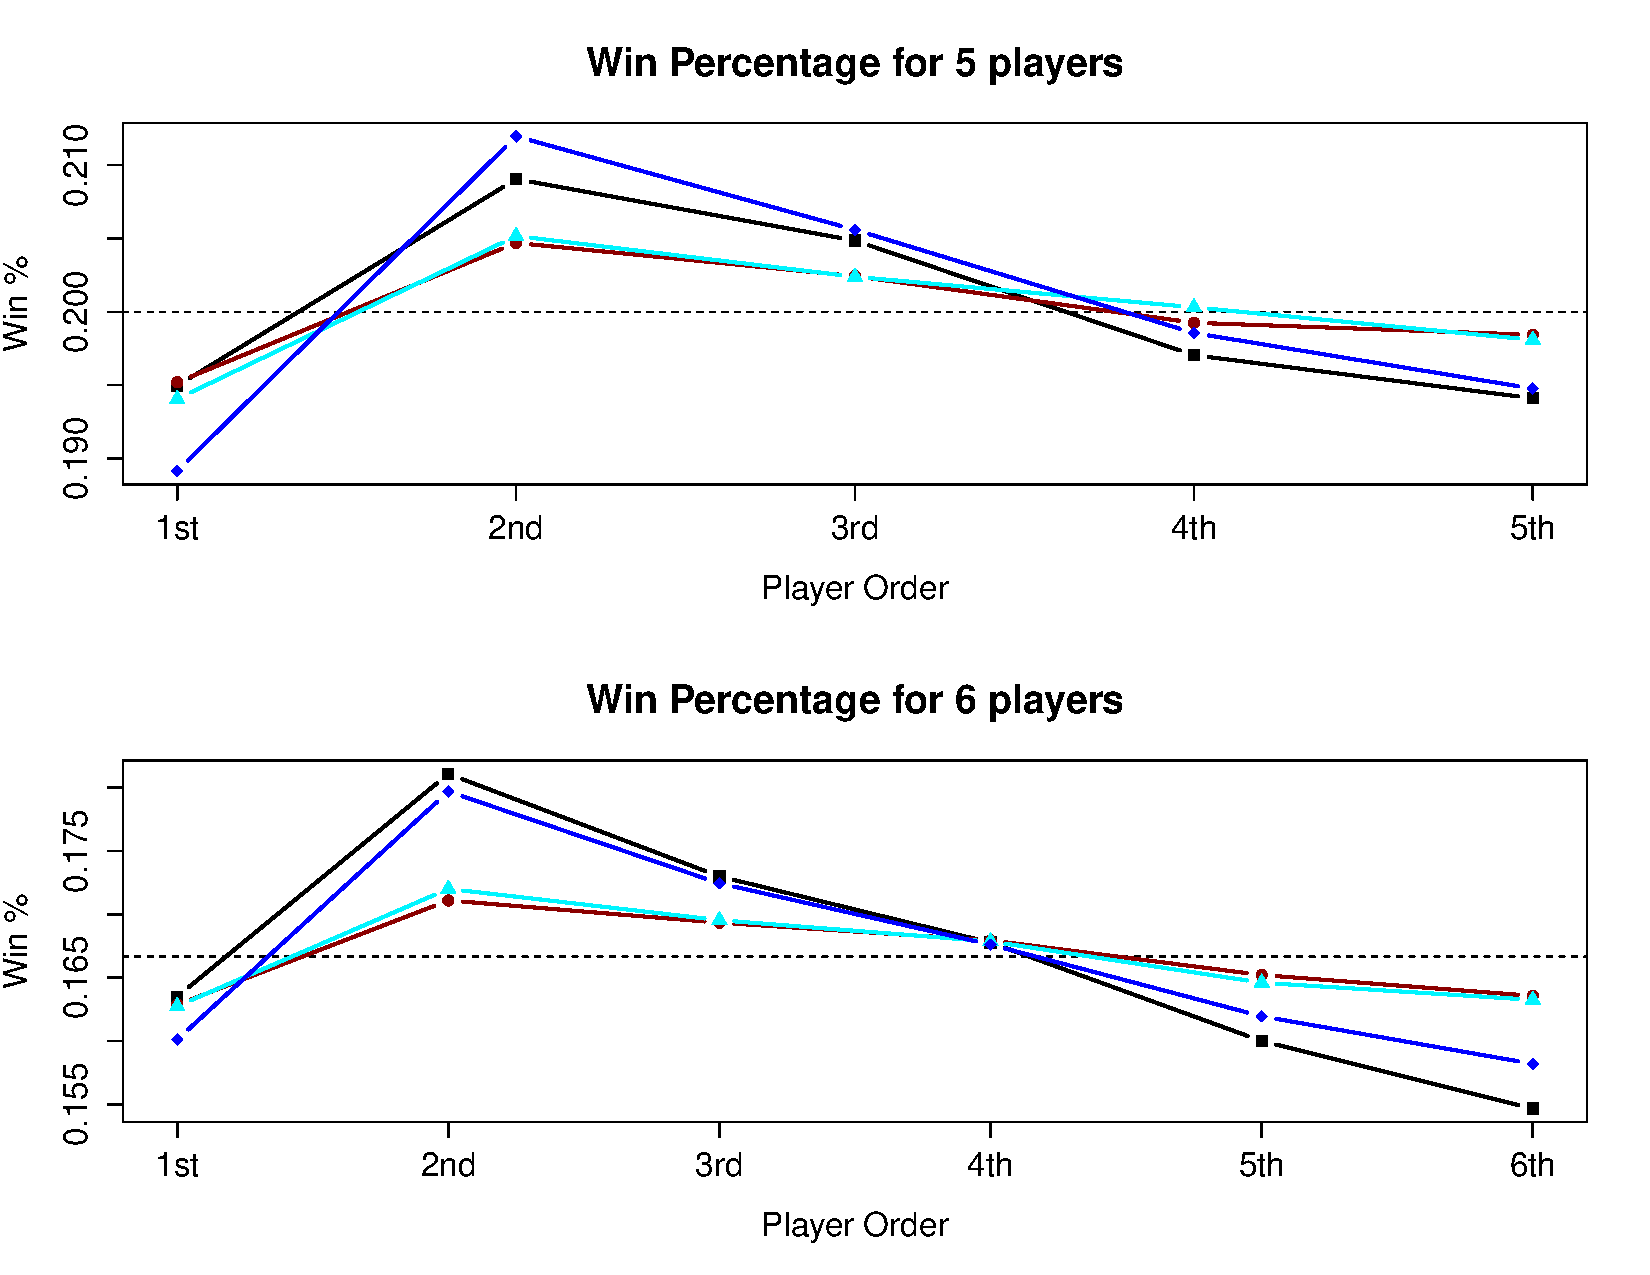
\includegraphics[scale=0.45]{imgs/win_5_6.pdf}
\end{figure}

\begin{figure}[h!]
	\centering
	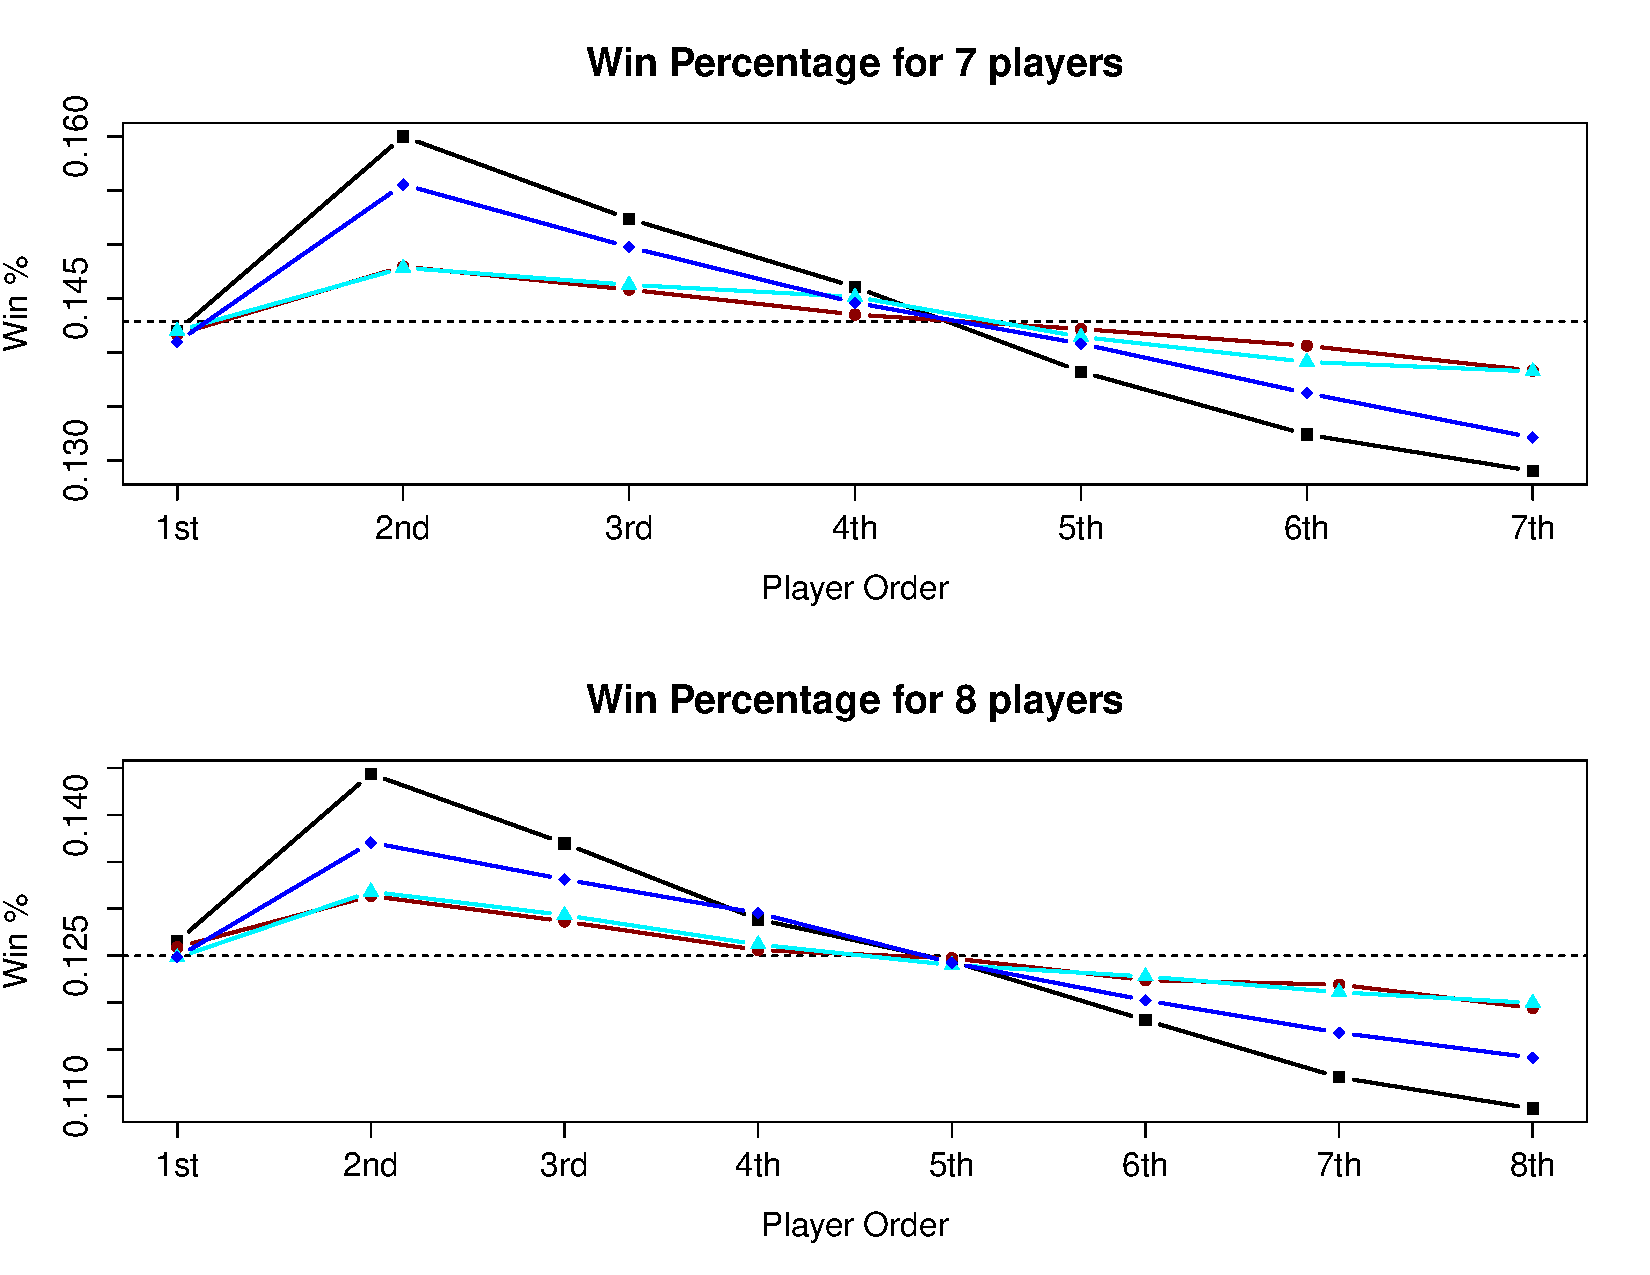
\includegraphics[scale=0.45]{imgs/win_7_8.pdf}
	\caption{\small Each plot shows the winning percentages of all four simulated variants for a given number of players. The dotted horizontal line marks what would be a perfect balanced game. This means that curves closer to that theoretical line are more balanced than others.}
    \label{fig:win_percents}
\end{figure}

Looking at these plots, the most striking feature is the second player constant advantage, regardless of the number of players or which game variation is being played. The third player also has some advantage but it's milder. Also surprising is the disadvantage of the first player that only achieves mean performance with seven and eighth players. Perhaps not so surprising is the disadvantage of the last players, especially in game with six players or more, given that when they start, the game has already several tokens in the board.

These plots confirm the better results of the Game of Goose, since its lines are closer to the theoretical best result -- the dotted black line where all players would lie if all had the same winning percentage. Also, the worst results from the game of Universe and the abstract variant can be seen here too, since their slopes are more steep, giving larger advantages for the second and third players -- and thus making these two variants less fair to play.

To confirm that the second player advantage is not a product of random noise, we tested these numbers against an uniform distribution of values -- which would be the appropriate statistical model for a perfect balanced race game, let's denote it a \textit{balanced variant} --, to see if the difference between the theoretical value and the simulated one were indeed significant. For each pair variant/number of players, we made a trial of 40000 matches of this \textit{balanced variant} and computed the ratio between the player with more wins against the player with less wins. These ratios simulate the outcomes of a perfect fair game\footnote{Notice that we did not play a game here. For $n$ players, we just sampled numbers from a uniform distribution between $1$ and $n$ and assigned the outcome $i$ as a win for the $i^{th}$ player}. We repeated this procedure 2000 times to reduce variation. Then, given these values, we found at which percentile our results fitted among these 2000 balanced outcomes. This implies that a value near than percentile $100$ means that our result is non uniform with high significance (i.e., some player(s) has advantage over others). We determined the threshold at percentile $90$. Less than this value is interpreted as not providing enough evidence to reject the hypothesis that a given variant is a fair game.

Figure~\ref{fig:win_percentiles} shows the computed percentiles:

\begin{figure}[h!]
	\centering
	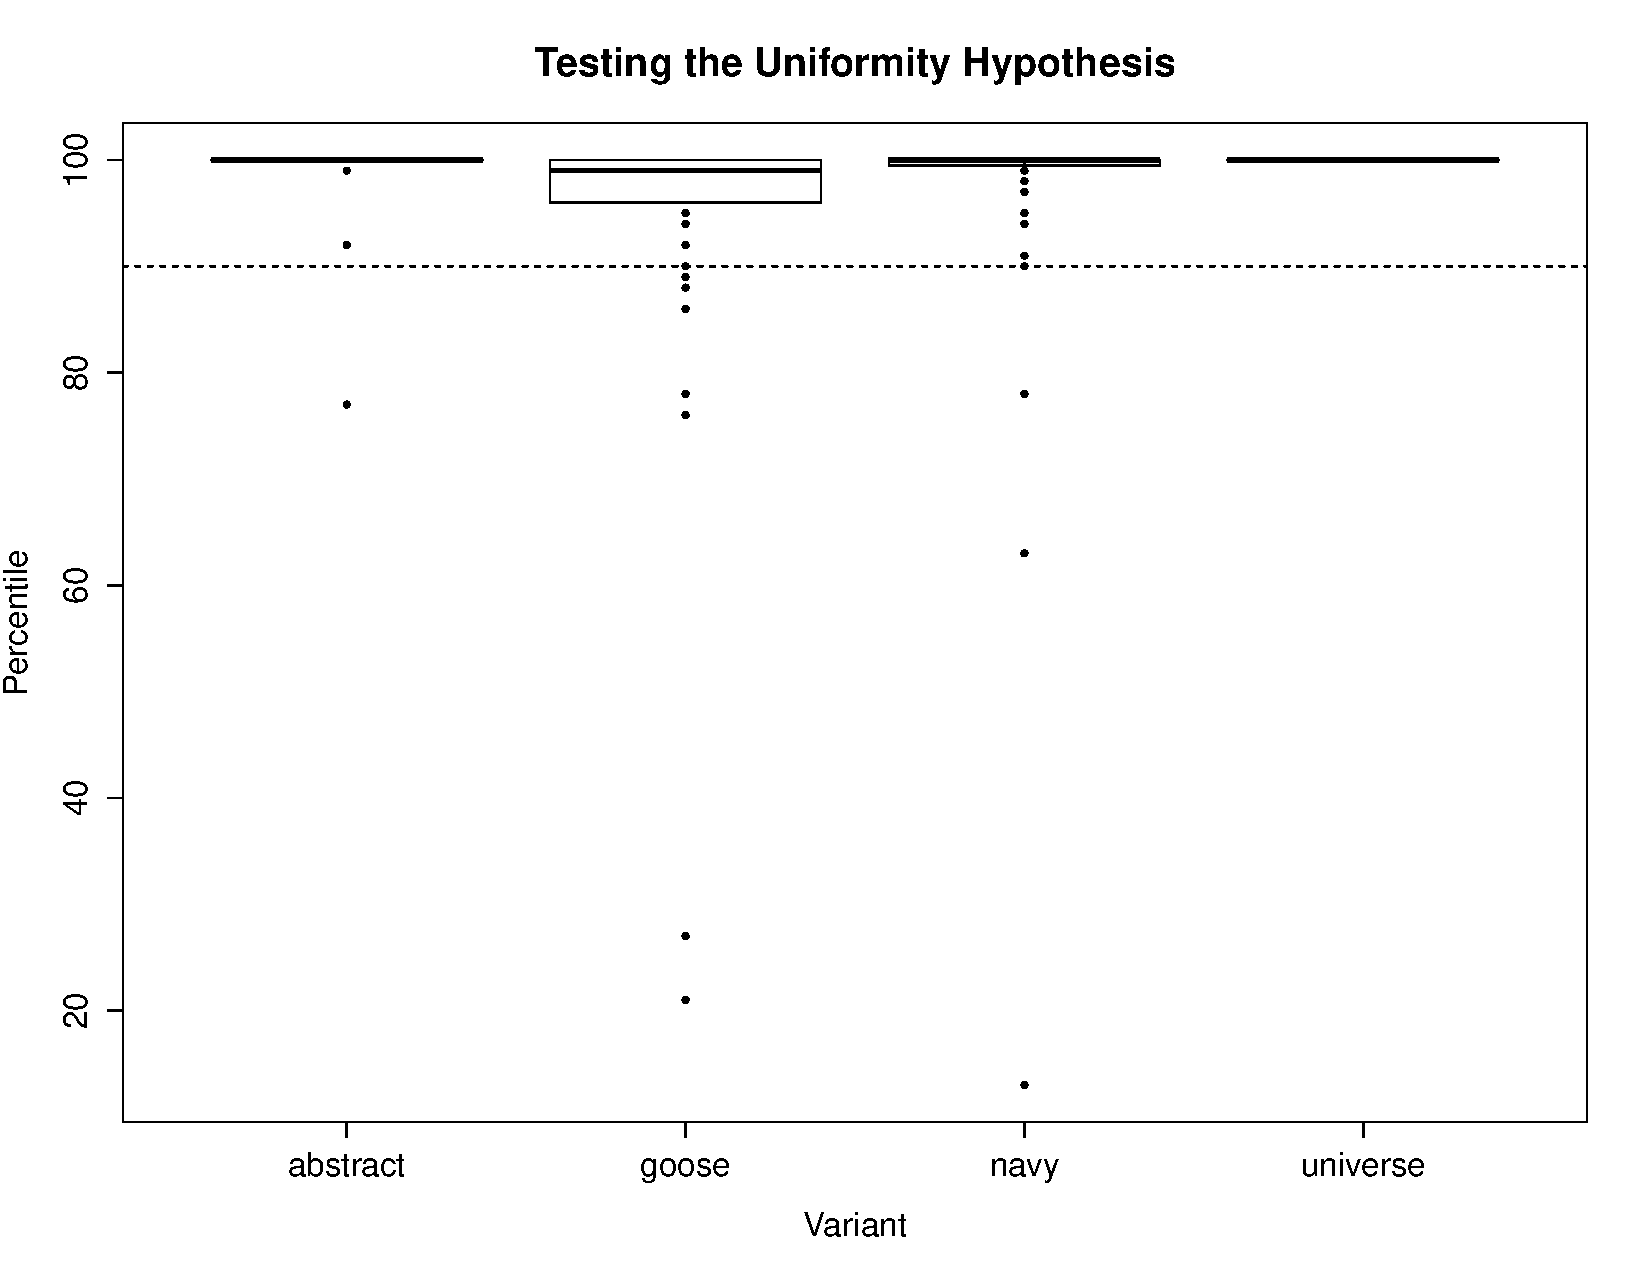
\includegraphics[scale=0.45]{imgs/win_percentiles.pdf}
	\caption{\small These are statistical box plots. The box represents the interquartile range, IQR, i.e., the values from percentile $25$ and $75$ (the bold line represents the sample median). Notice that for all but the Game of Goose, the stability of the results produced a IQR so small that it collapsed the box into a line. The points represent values outside IQR. The dotted line marks the chosen threshold at percentile $90$.}
    \label{fig:win_percentiles}
\end{figure}

There are 36~trials for the abstract variant, and 72~trials for each of the historical games. The values below the dotted line could be interpreted as evidence for the uniform hypothesis (except for the game of Universe that does not have a single outlier). However, the great majority of the results were placed at percentile~100 or at very high~90s, which is a strong evidence for the non-uniformity hypothesis. This data, together with the previous plots, presents a convincing argument for the second player advantage in these four variants.

However, even if these variants present players initial advantages, the difference between the estimated best and worst players is not that large. The maximum differences are around three percentage points, which is not enough to impact on the game play of occasional players. Seasoned players might notice this, but can easily fix this problem by rotating among themselves which one is the first player to start.

\subsection{\lead~criteria}

\lead~values state that a game is more dramatic if the player that wins did achieve the lead only a few turns before the end of the game. In the following simulations we measured the lead up to five turns before the end of the variant. Again, we did this for each variant and each number of players (from three to eight).

\begin{figure}[h!]
	\centering
	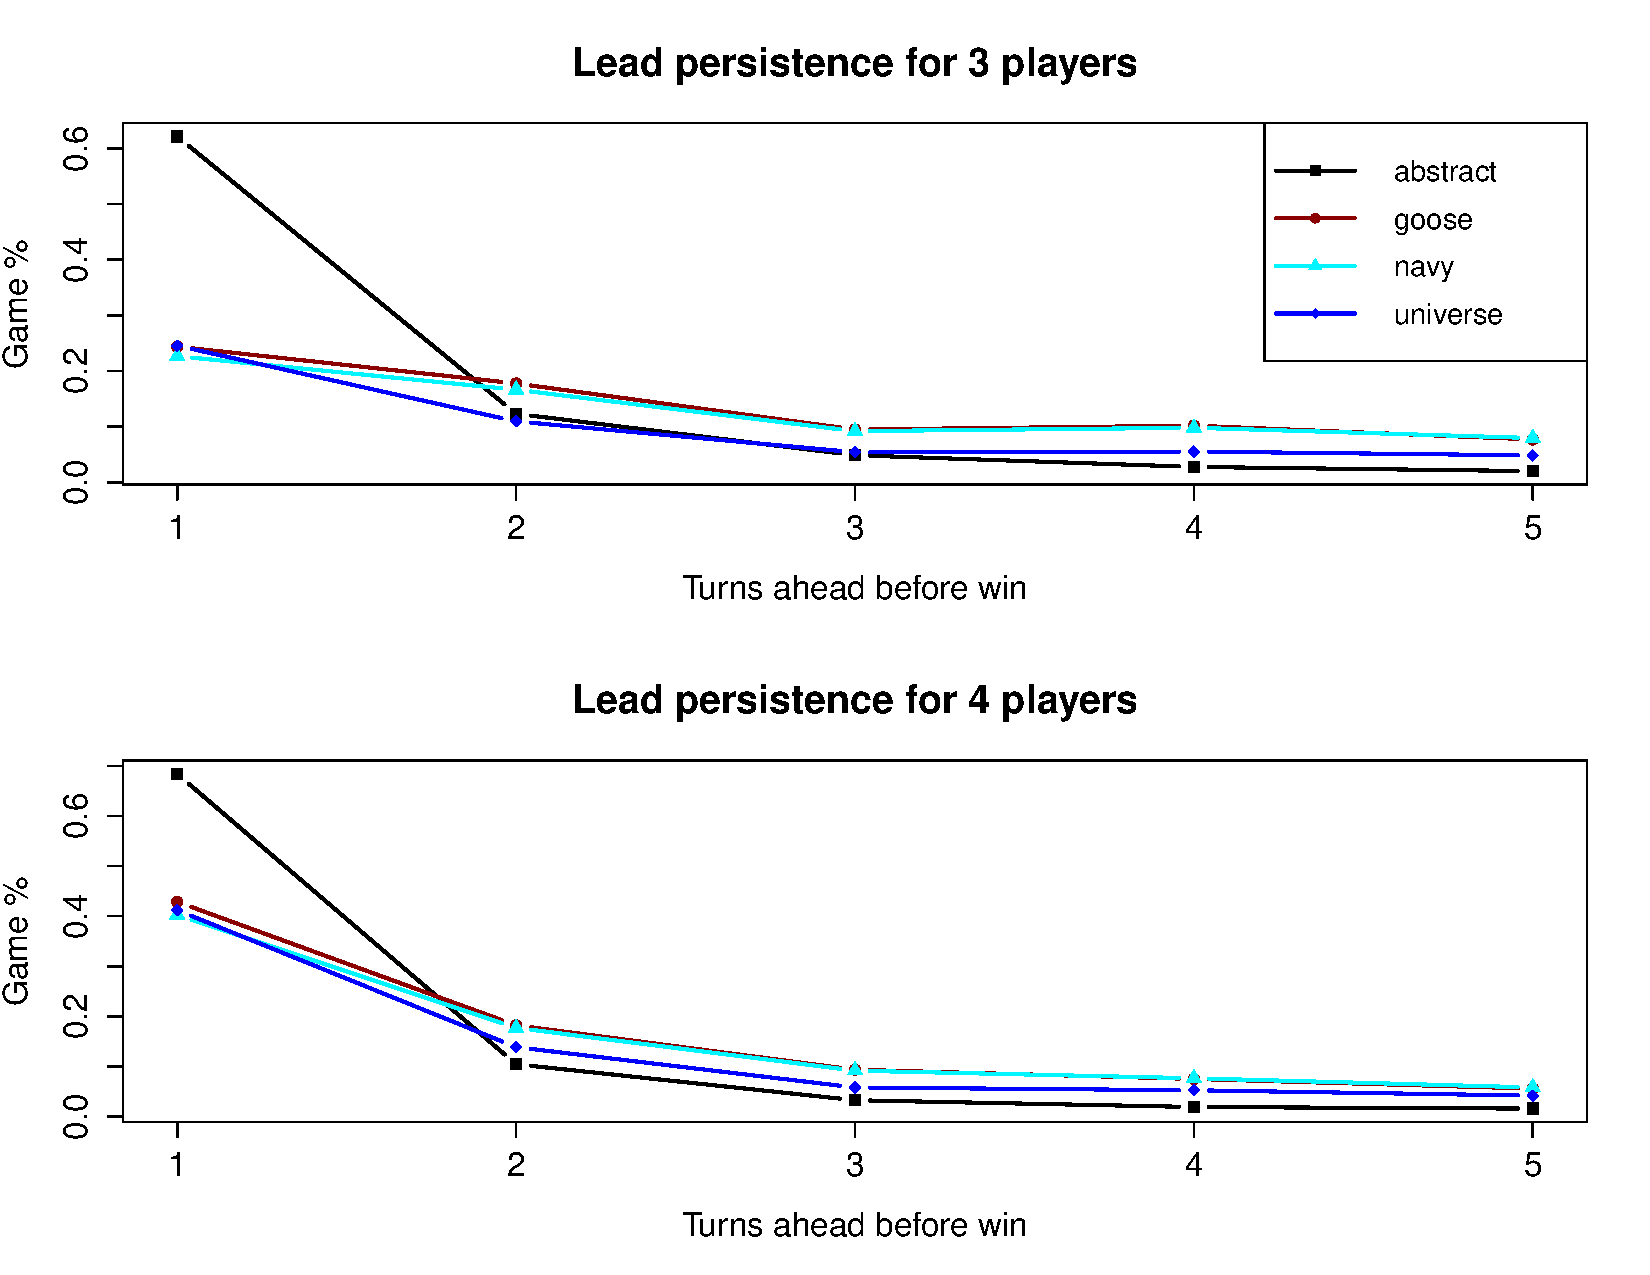
\includegraphics[scale=0.4]{imgs/lead_3_4.pdf}
	\caption{\small Each plot shows what the match percentage where the winner had the lead for one to five turns at the end. As an example for 3 players, the abstract variant, in 61\% of the matches, found its winner only at the last turn, i.e., the majority of matches had seen a leader reversal just at the last moment. This implies good drama from a \lead~perspective.}
    \label{fig:lead_percents}
\end{figure}

\begin{figure}[h!]
	\centering
	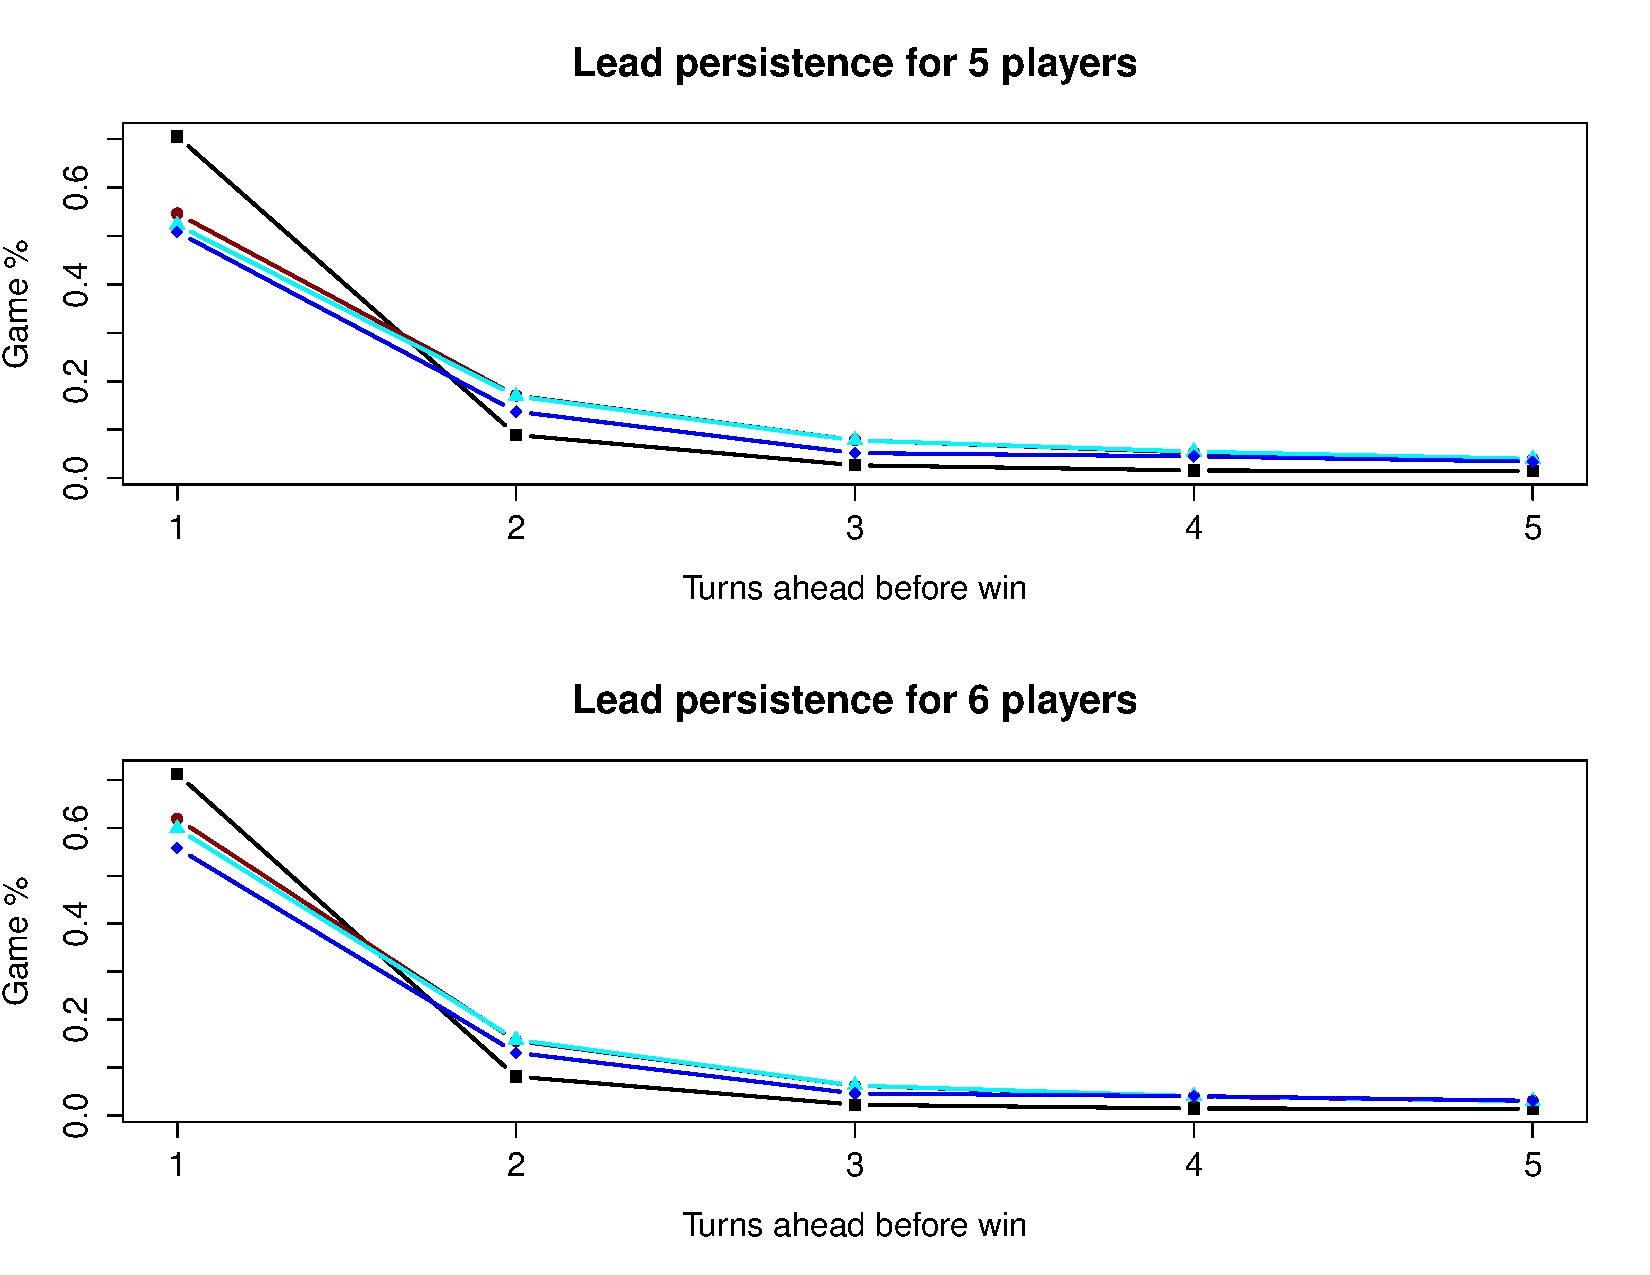
\includegraphics[scale=0.4]{imgs/lead_5_6.pdf}
\end{figure}

\begin{figure}[h!]
	\centering
	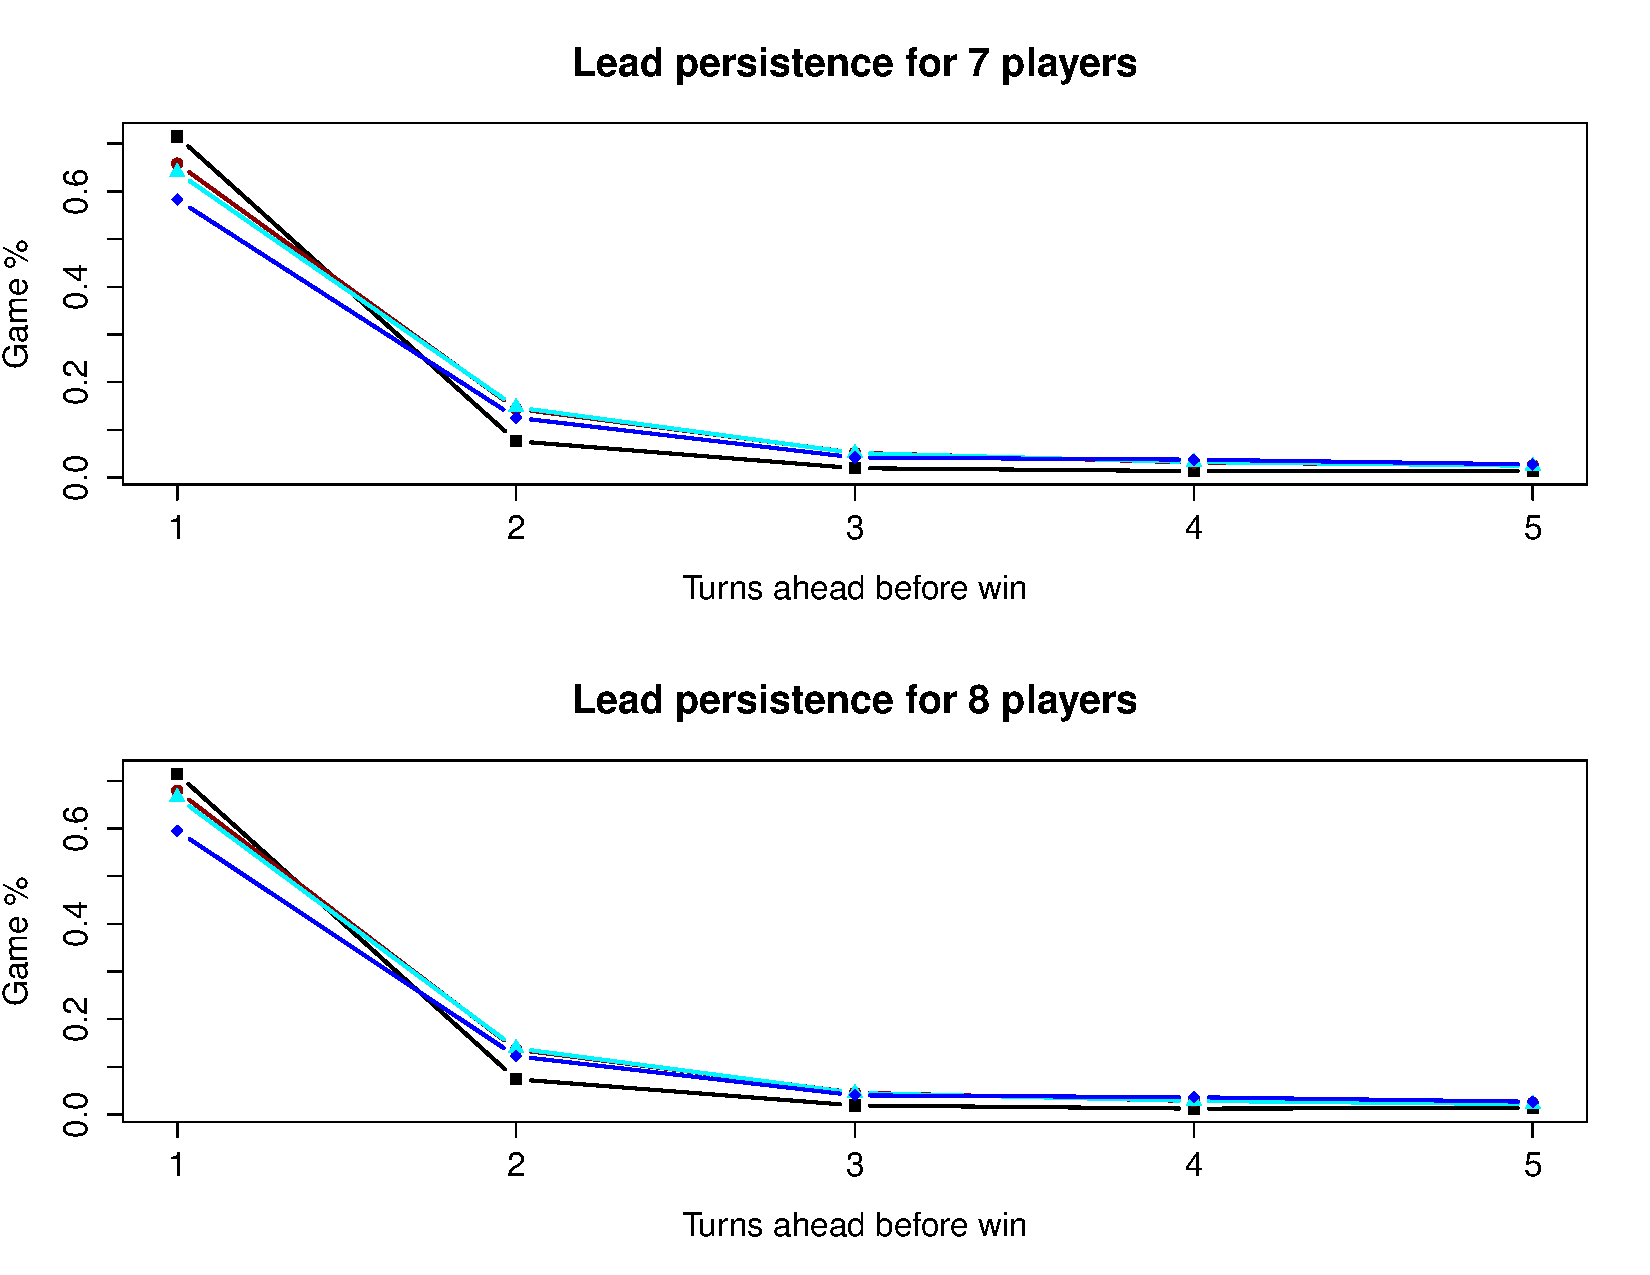
\includegraphics[scale=0.4]{imgs/lead_7_8.pdf}
\end{figure}

The abstract variant is the most dramatic by this criteria. Even for three players, the games where the winner just got his lead in the last turn is more than $60\%$. However this difference get smaller and smaller as we add more players. With six players the distributions for all four games are quite similar. Comparing the three historical games, the Game of Goose is slightly better than the other two, but this difference might not be significant despite the number of matches we are dealing with.  

Among all games, the abstract version had $84\%$ of games with up to five turns ahead for the winner, the Goose had $86\%$, the Navy $84\%$ and the Universe $74\%$. This means all variants are quite dramatic by this criteria. They do not frequently produce matches where the winner is known many turns before the endgame. Only one sixth to one forth of the games the lead is kept for more than five turns. Curiously, if these percentages were more extreme, say, 95\% of matches are won at the last moment, the drama would also be hard to keep: players would rightly guess that the current lead would not win. As it is, the players still have plenty of room for doubt, which is a good feature for a race game.

\subsection{\anp~criteria}

The \anp~criteria focus on the number of different players that were ahead during a game. The argument is that a game is more dramatic the more players are able to take the lead. A game where the first player leading maintains her lead during the entire match is arguably less dramatic than one where there are many players able to be ahead of the others during the match. The mean values of all trials are presented at figure~\ref{fig:anp_leads}.

\begin{figure}[h!]
	\centering
	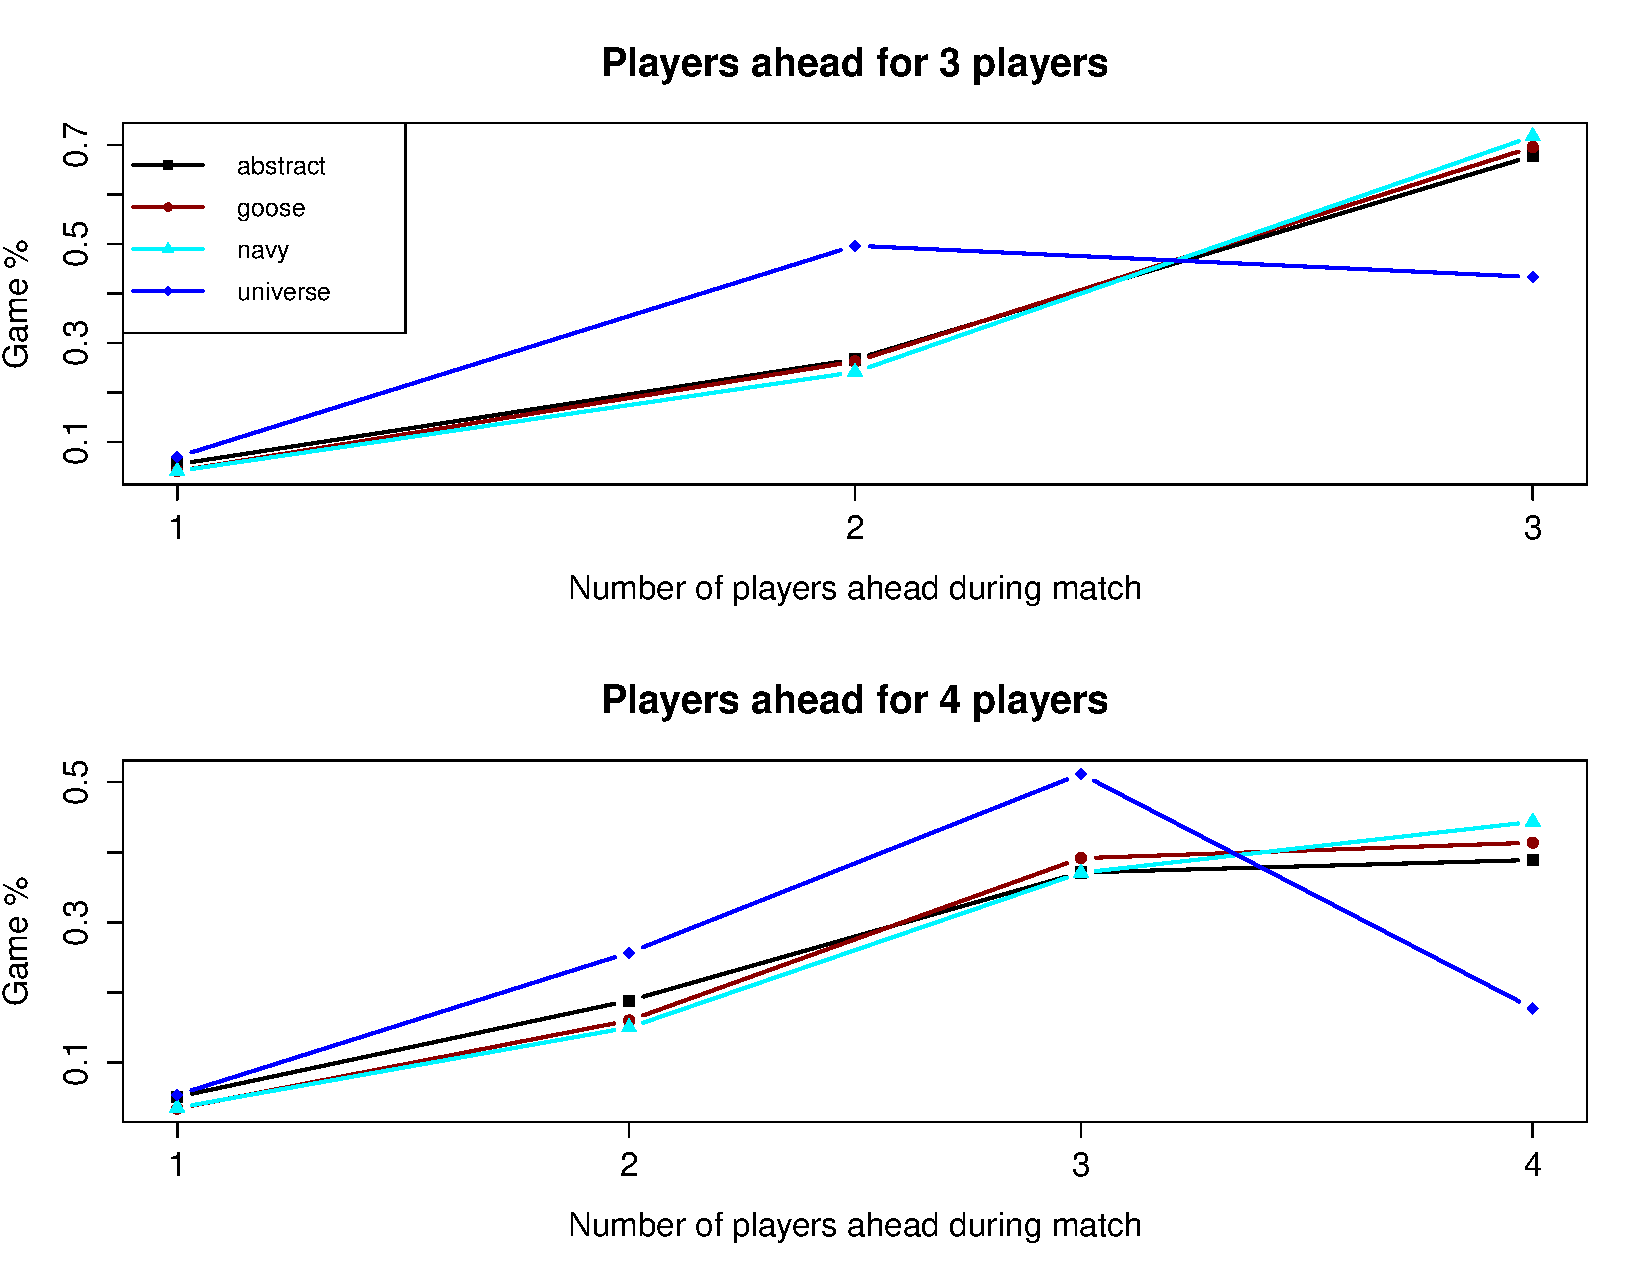
\includegraphics[scale=0.45]{imgs/anp_3_4.pdf}
	\caption{\small Each plot shows, for each game and for $n$ players (again, $3\leq n\leq 8$), the percentage of games where the number of leaders were $1$ to $n$. As an example, the Game of Universe with 3 players had around $50\%$ of the matches with two different leaders.}
    \label{fig:anp_leads}
\end{figure}

\begin{figure}[h!]
	\centering
	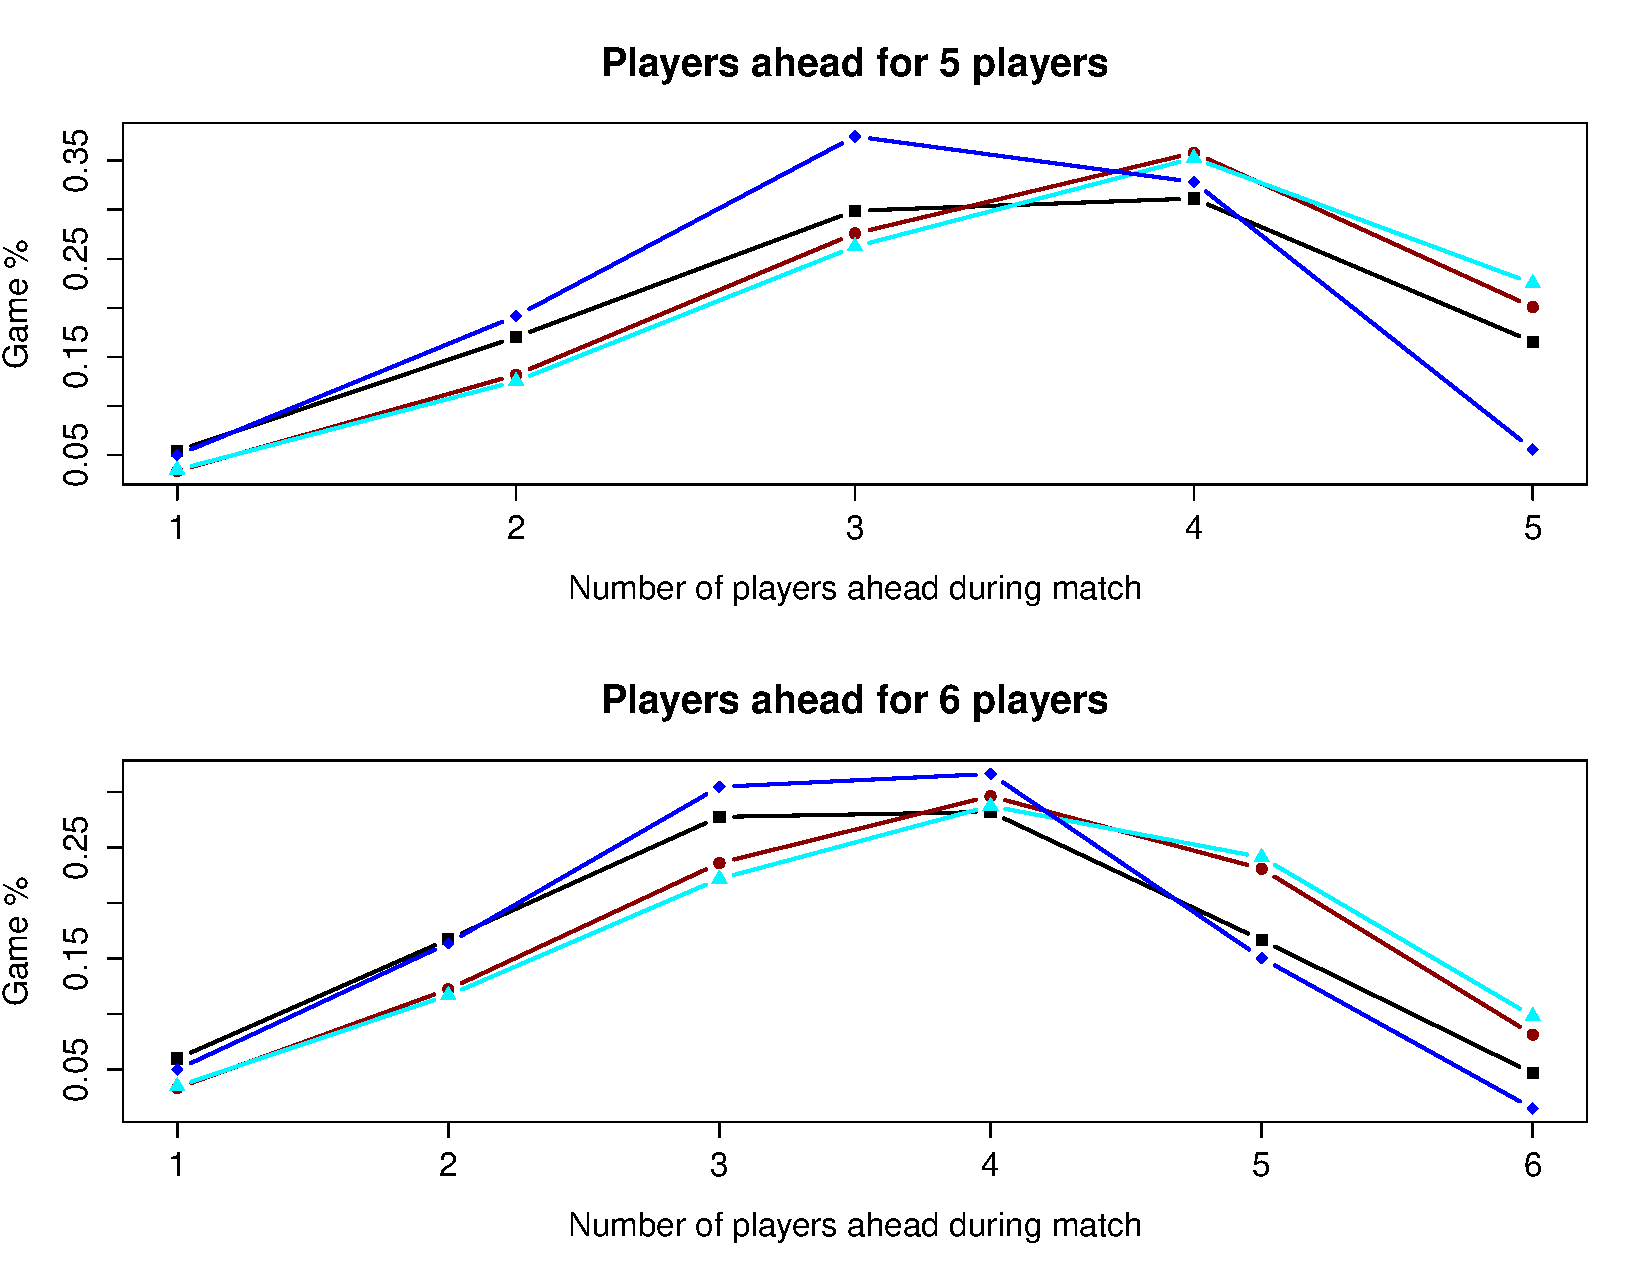
\includegraphics[scale=0.45]{imgs/anp_5_6.pdf}
\end{figure}

\begin{figure}[h!]
	\centering
	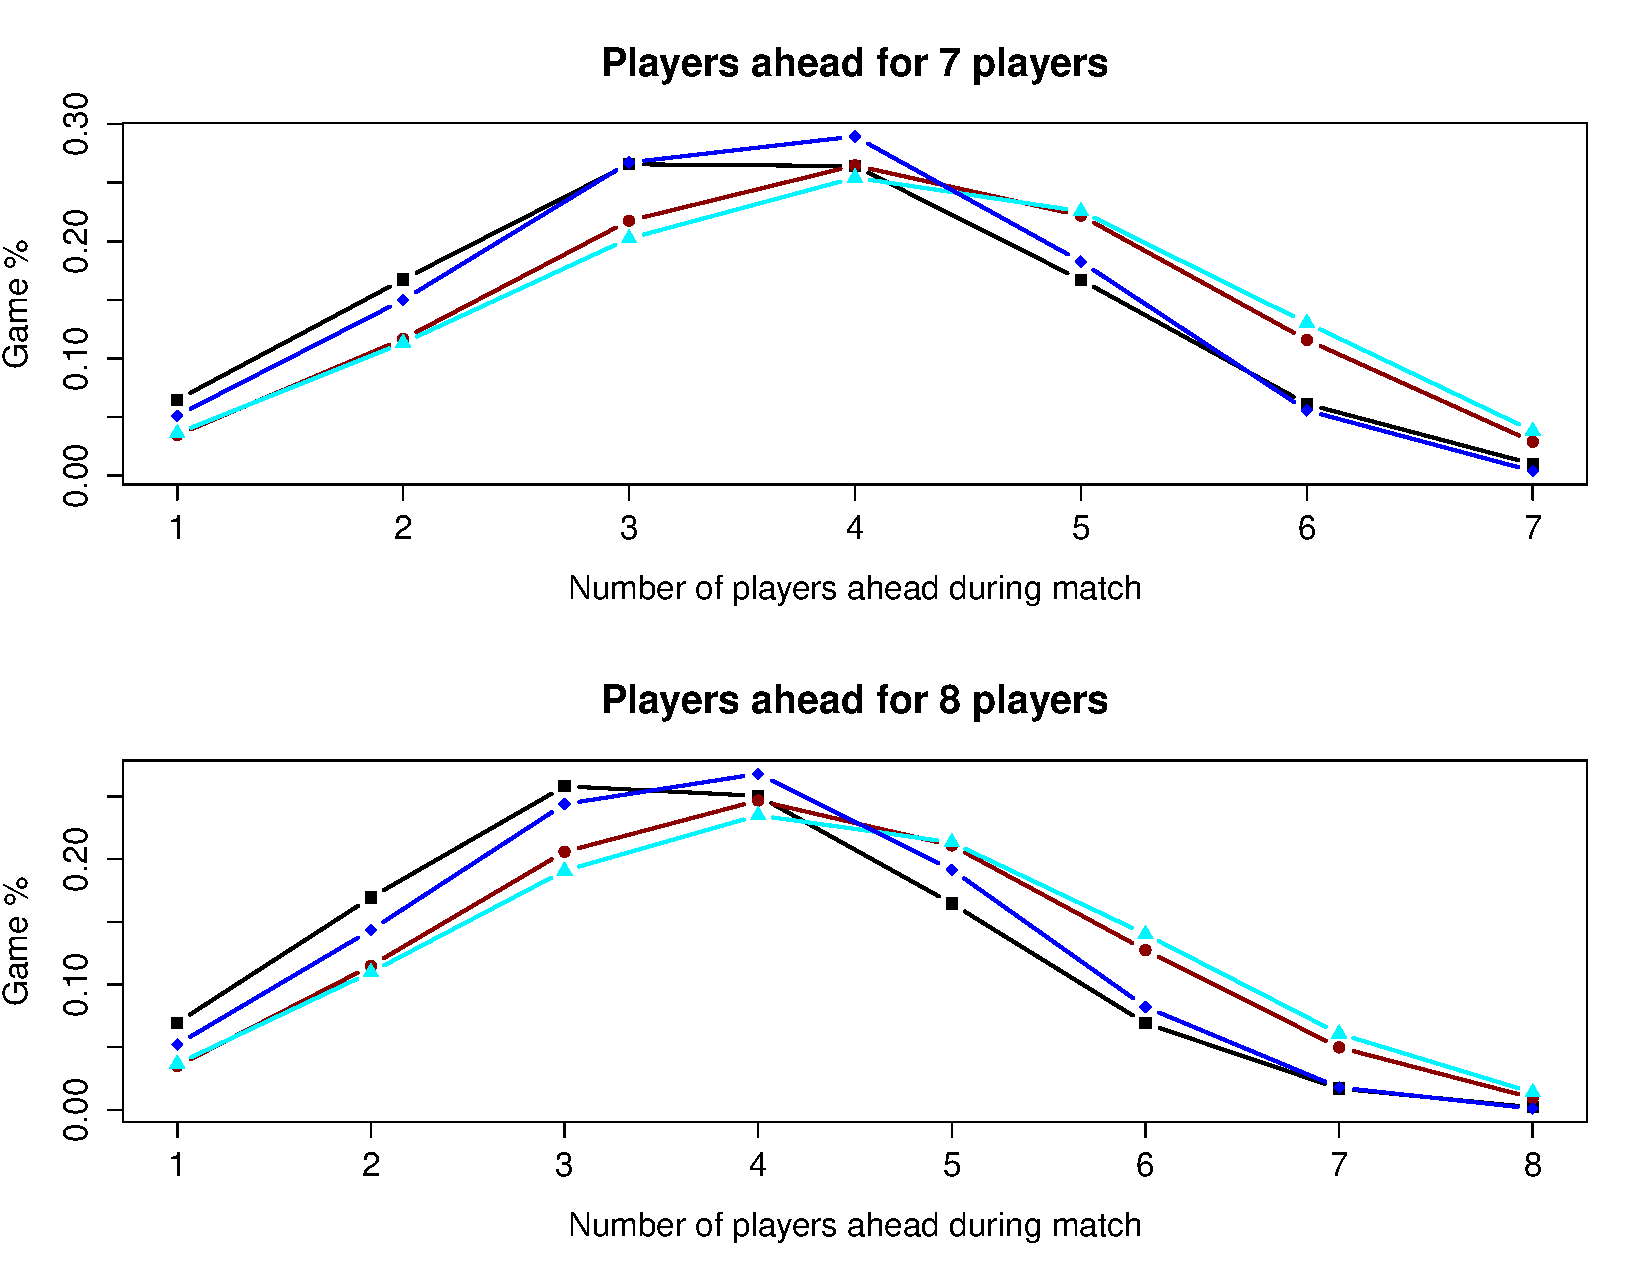
\includegraphics[scale=0.45]{imgs/anp_7_8.pdf}
\end{figure}

For all variants the amount of matches with a single lead is quite small, less than $5\%$ of the games are like that. The data shows that in the typical match, with at least four players, about half the players take the lead. This is a good balance. A game where, on an average match, all the players are ahead might feel a bit too chaotic (and indeed, there are very few of those). But a game where about half the number of players take the lead provides, in our perspective, a good gaming experience.

Comparing games, the game of Universe is the less dramatic for three or four players, but behaves quite similarly with the others if the number of players are five or more. For many players, the Game of Goose and the Game of Navy are the ones that allow more lead changing events.

\subsection{Match Size}

This experience provided with more data besides the evaluation of the three drama criteria. Another feature, not related to drama, but important in gaming experience, is the average match length. If too short or too long matches are frequent, the game becomes boring and dull. However, if the average length is usually socially admissible\footnote{The range of admissible turns a game should have depends on the culture embedding it. It is quite possible that if Go was invented today it would not have succeeded given the great amount of turns needed to complete a match (around 300 to 400 stone placements).}, the fact of having some rare matches ending too soon or taking too long, might be interpreted as a game bonus and played with increased interest.

\begin{figure}[h!]
	\centering
	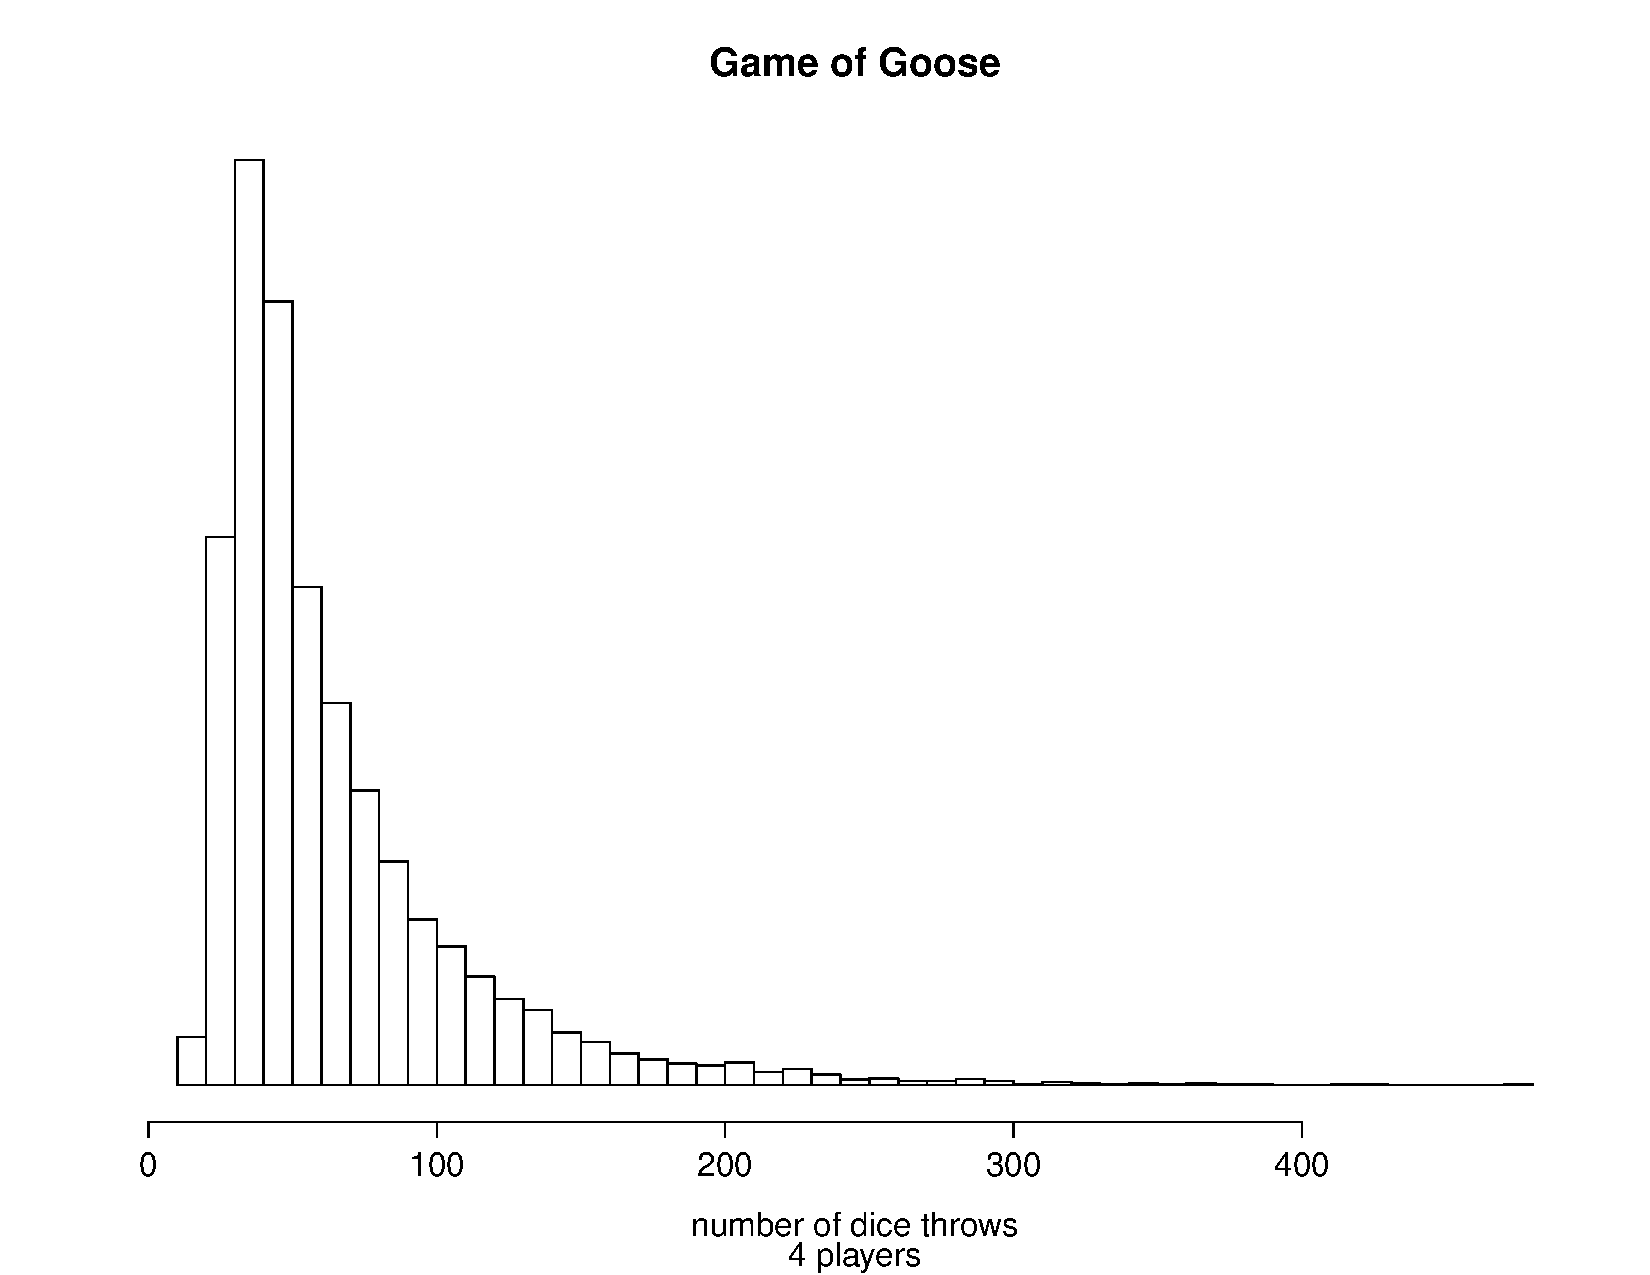
\includegraphics[scale=0.35]{imgs/goose_histogram.pdf}
	\caption{\small This plot shows the histogram of the number of needed dice throws to end 12500 games of Goose with four players. Herein, a turn consists of four dice throws, since there are four players.}
    \label{fig:goose_histogram}
\end{figure}

\begin{figure}[h!]
	\centering
	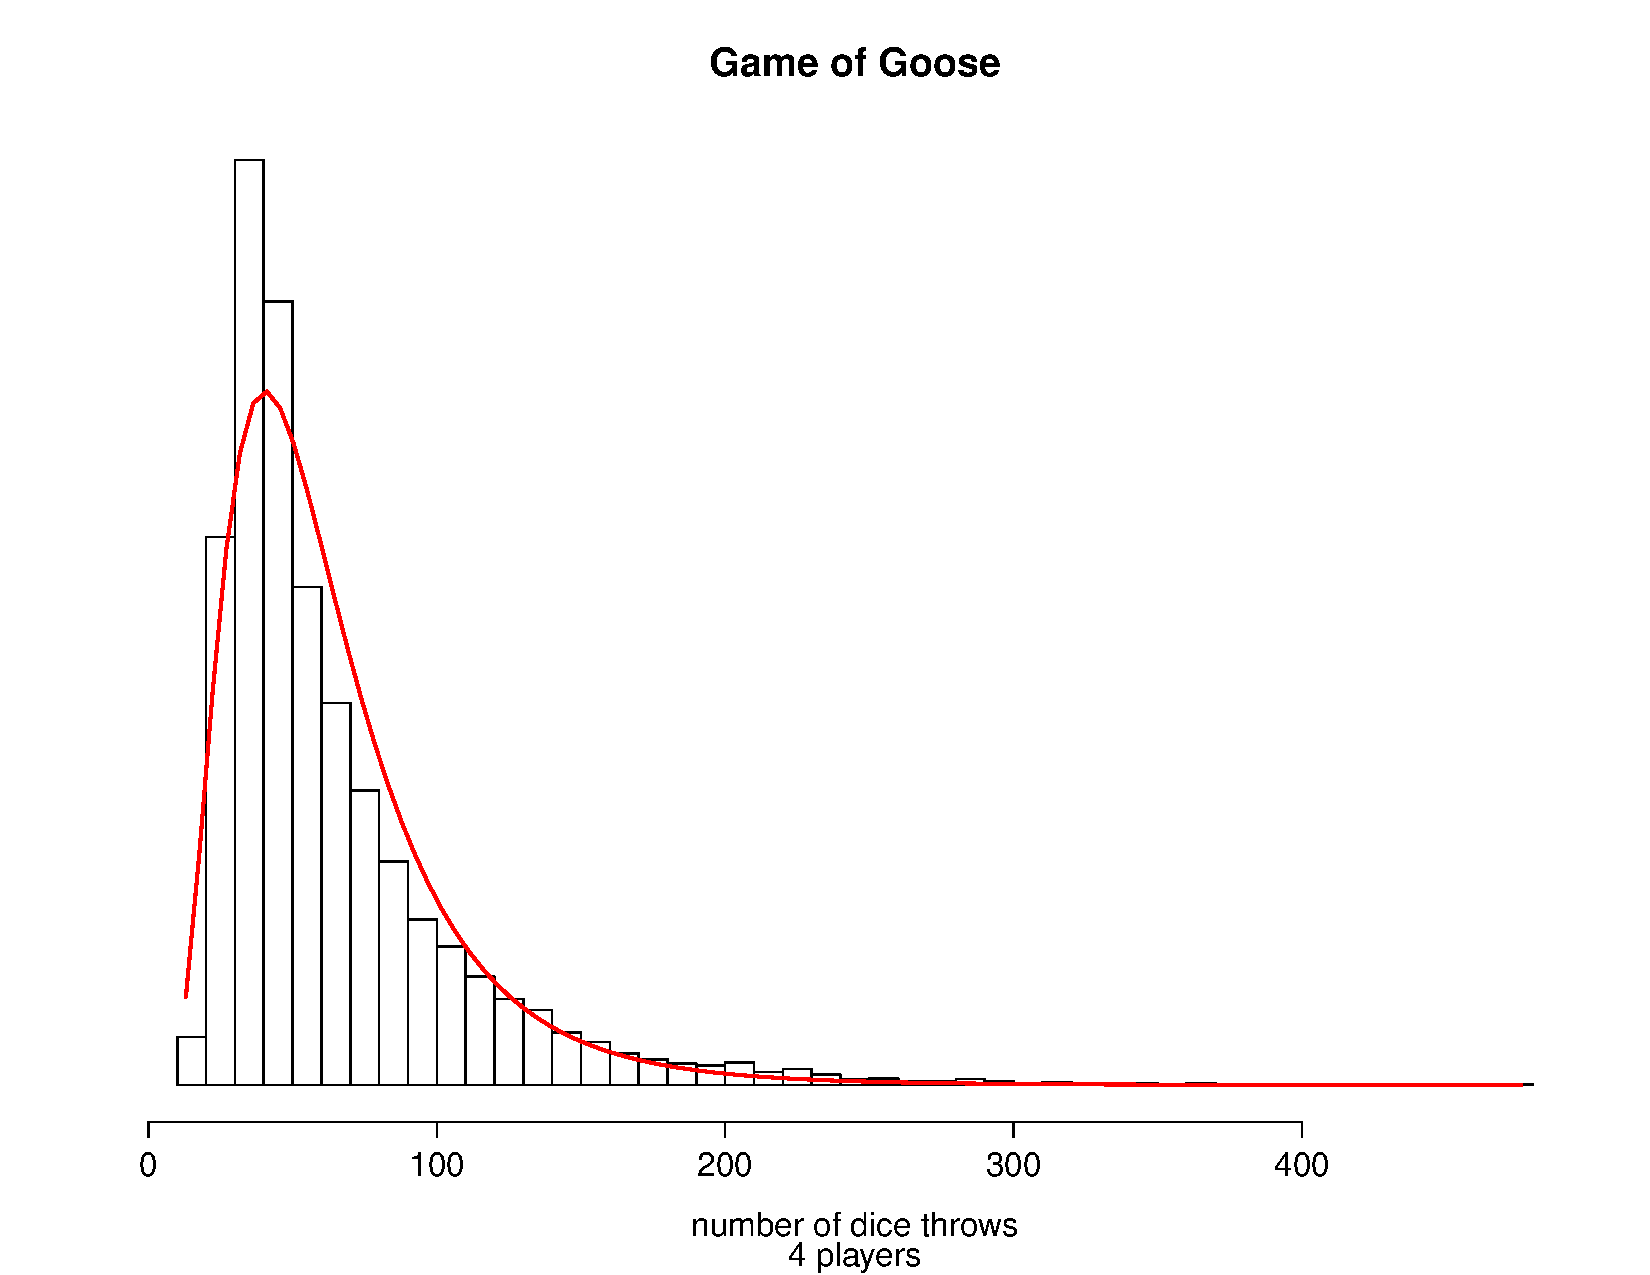
\includegraphics[scale=0.35]{imgs/goose_fit.pdf}
	\caption{\small This plot shows the previous histogram with the best log-normal fit.}
    \label{fig:goose_fit}
\end{figure}

Figure~\ref{fig:goose_histogram} shows an histogram of the distribution of game moves for 12500 games of four player Goose. The histogram has the shape of an asymmetric distribution with an heavy tail to the right: some games takes many hundreds of moves to end. Disregarding this tail, i.e., rare matches that take too long due to a great number of consecutive traps and captures, the histogram shape is quite close to a log-normal distribution. Figure~\ref{fig:goose_fit} shows the best fit for a log-normal. This fit also works nicely to all the historical variants as well to the abstract variant.

This relationship with the log-normal is just an empirical statement. We do not know a formal argument  relating this well-known distribution to the number of moves necessary to end a Goose-like race game. It is quite possible that more Goose variants also share this pattern, and it should be an interesting subject to determine if this pattern also arises in other race-like games.

The trials computations kept all fit values which we are able to plot them together in figure~\ref{fig:log_fits}.

\begin{figure}[h!]
	\centering
	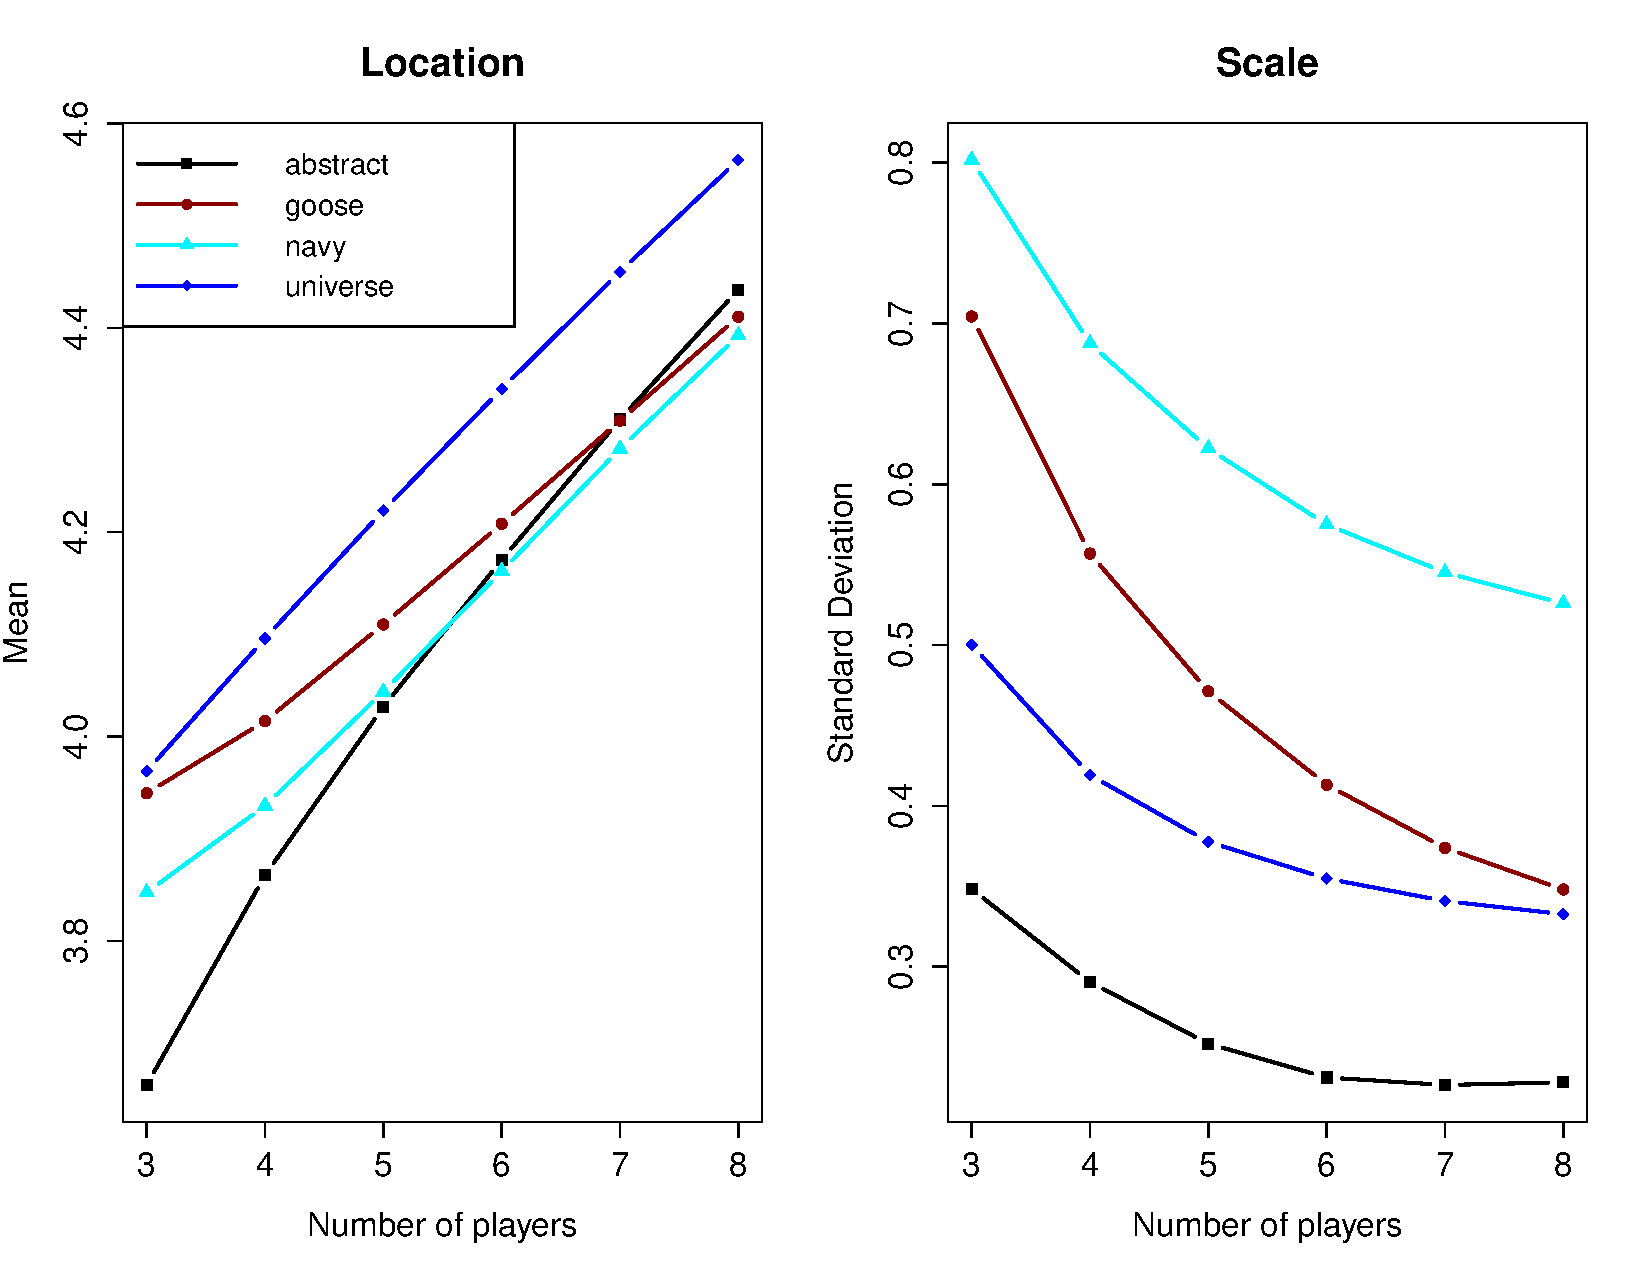
\includegraphics[scale=0.45]{imgs/log_fits.pdf}
	\caption{\small A log-normal distribution has two parameters: i) a location parameter that specifies the distribution's mean, and ii) a scale parameter that specifies how much spread we should expect. This pair of plots show, for each variant, how these parameters change accordingly to the number of players.}
    \label{fig:log_fits}
\end{figure}

According to figure~\ref{fig:log_fits}, all variants despite having quite different parameters regarding their special rulings (e.g., where are the traps, where and how are the jump spaces), share a similar behaviour concerning the log-normals fits. The location trend suggests that Goose-like variants with more players tend to take longer to finish, which is an expected result. The scale trend, however, suggests that the expected variation of the number of turns tends to be smaller as the number of players increase, which is not an obvious consequence, even if it seems to stabilize after a certain amount of players (its exact number depends on the variant). Both trends are well-behaved. This is evidence that it should be possible to achieve good estimations for the expected number of moves, given the number of players. 

\end{document}
